\documentclass{article}
\usepackage[utf8]{inputenc}
\usepackage[T1]{fontenc}
\usepackage{graphicx}
\usepackage{subfiles}

\begin{document}
\section{Arhitektura sistema}
\subsection{Kratak opis arhitekture}
Pri razmatranju tipa arhitekture sistema izabran je troslojni dizajn arhitekture:
\begin{enumerate}
    \item \textbf{Prezentacioni sloj}
    \item \textbf{Logički sloj}
    \begin{enumerate}
        \item\textbf{Klijent kontroler}
        \item\textbf{Server kontroler}
    \end{enumerate}
    \item \textbf{Sloj podataka}
\end{enumerate}

Za tip aplikacije je izabrana Veb aplikacija koja podrazumeva jedan server i više klijenata, zbog čega je, radi stabilnije komunikacije i boljeg korisničkog iskustva, izabran MERN Stack za njenu implementaciju: 
\begin{enumerate}
    \item \textbf{MongoDB} - Sloj podataka
    \item \textbf{Express.JS} - Server kontroler
    \item \textbf{React.JS}\begin{itemize}
        \item Prezentacioni sloj (uz to podrazumevaju se i HTML, CSS, JavaScript)
        \item klijent kontroler
    \end{itemize} 
    \item \textbf{Node.JS} - Server kontroler

\end{enumerate}
Ovim smo omogućili kreiranje dinamičke "single-page" veb aplikacije sa kompleksnim interfejsom, a jednostavnim komponentama. Ima odličnu podršku za forme, regulisanja grešaka, kalendara, lista i još mnogo toga. 

\newpage
\subsection{Dijagram arhitekture sistema}
\begin{figure}[!ht]
        \begin{center}
            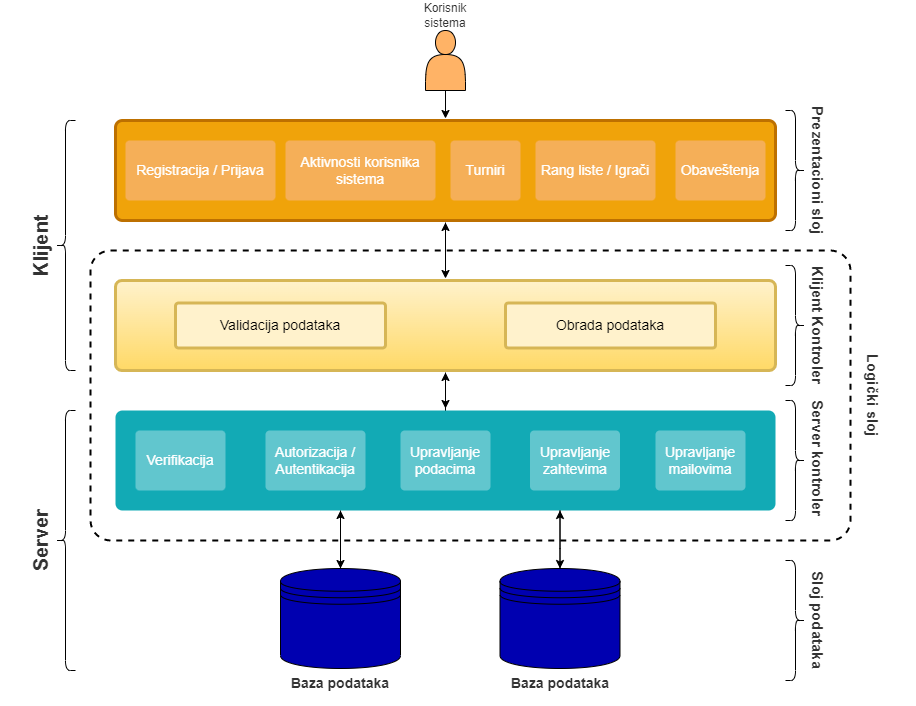
\includegraphics[scale=0.45]{Arhitektura/Dijagrami/Arhitektura.png}
        \end{center}
    \caption{Dijagram arhitekture sistema}
    \end{figure}

\begin{itemize}
    \item Prezentacioni sloj je ono što svi korisnici mogu da vide (registrovani i neregistrovani). Neregistrovanom su dostupne informacije o turnirima, rang listama i igračima, kao i obaveštenja, dok za registrovane imamo deo koji spada u "Aktivnosti korisnika sistema" i to su specijalni slučajevi na osnovu rezultata autorizacije/autentikacije i uloga u sistemu.
    \item Klijent kontroler je sloj koji na tom najvišem nivou proverava ispravnost unetih parametara, sa prezentacionog sloja, u odre\dj ena polja i na kom se vrši i obrada podataka koji su prosle\dj eni od strane servera. 
    \item Server kontroler prihvata zahteve od klijentskog kontrolera, obradjuje primljene podatke i na osnovu toga izvršava neophodne zadatke u okviru sistema kao i neophodnu komunikaciju sa bazom podataka.
\end{itemize}


\newpage
\subsection{Dijagram implementacije arhitekture sistema}
\begin{figure}[!ht]
        \begin{center}
            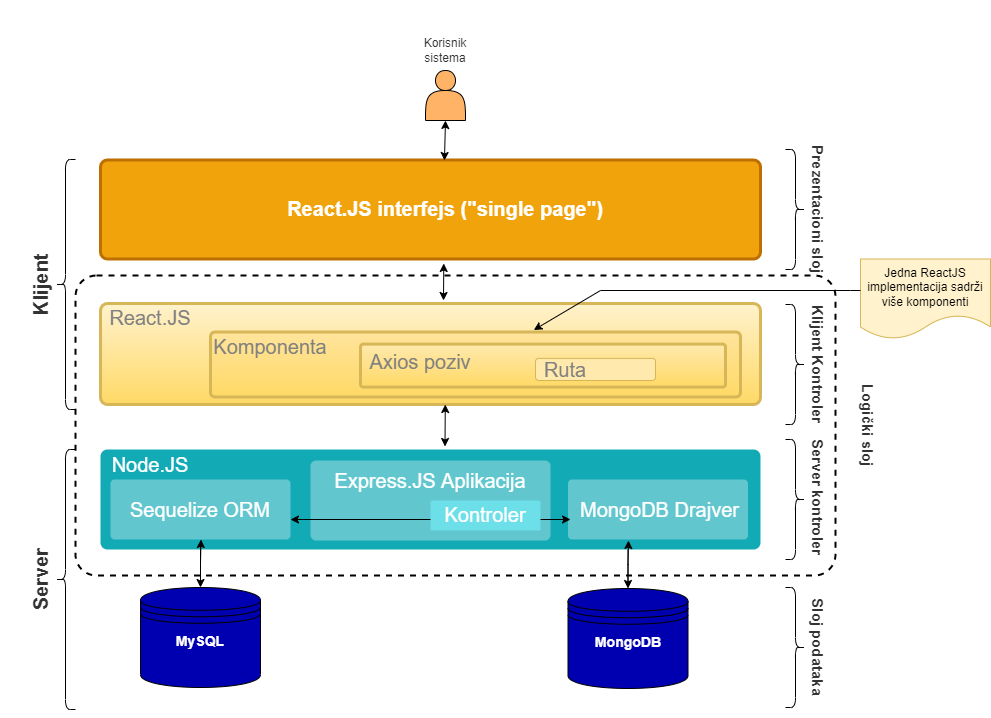
\includegraphics[scale=0.45]{Arhitektura/Dijagrami/Implementacija arhitekture.png}
        \end{center}
    \caption{Dijagram implementacije arhitekture sistema}
    \end{figure}
    
\newpage
\subsection{Dijagram isporučivanja}
\begin{figure}[!ht]
        \begin{center}
            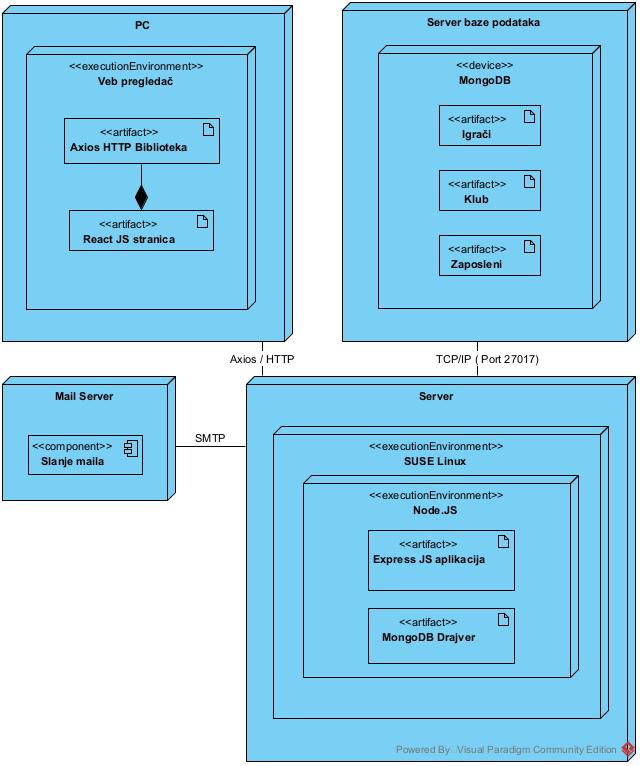
\includegraphics[scale=0.6]{Arhitektura/Dijagrami/Deployment Diagram.jpg}
        \end{center}
    \caption{Dijagram isporučivanja}
    \end{figure}
    
\newpage
\subsection{Dijagram komponenti}
Dijagram komponenti informacionog sistema tensiskog saveza se sastoji od 3 pod sistema:
\begin{enumerate}
    \item Nalozi,
    \item Turnir,
    \item Globalne informacije.
\end{enumerate}

U okviru podsistema Nalozi se nalaze komponente zaposleni i korisnici koje upravljaju nalozima i registracijama svih učesnika. Ove komponente pružaju interfejse koji su potrebni drugim podsistemima. Podsistem globalne informacije, koji je zaduđen za objavljivanje informacija, zavisi od komponente zaposleni koji pruža odgovarajući interfejs. On se sastoji od komponenti RangLista, Medicinska ustanova, Obaveštenja i Inforrmacije o turniru koji pružaju interfejse za uvid u informacije.

Turnir predstavlja podistem koji se bavi svim informacijama vezanim za turnire i njihovu organizaciju. Autentifikacija je komponenta koja proverava da li je ulogovani korisnik organizator i omogućava da samo on menja informacije vezane za organizaciju turnira. U Organizaciju turnira spadaju aktivnosti organizacije žreba, slanja specijalnih pozivnica, odlaganje turnira, odustajanje od organizacije turnira kao i prijava i odjava igrača za turnir. Komponenta meč omogućava upravljanje podacima vezanim za konkretan meč koje su potrebne za konačne rezultate na turniru. Komponenta rezultati pruža interfejs upravljanjaRezultatima koji omogućava pravilno formiranje RangListe i njen prikaz.


\begin{figure}[htbp]
        \begin{center}
            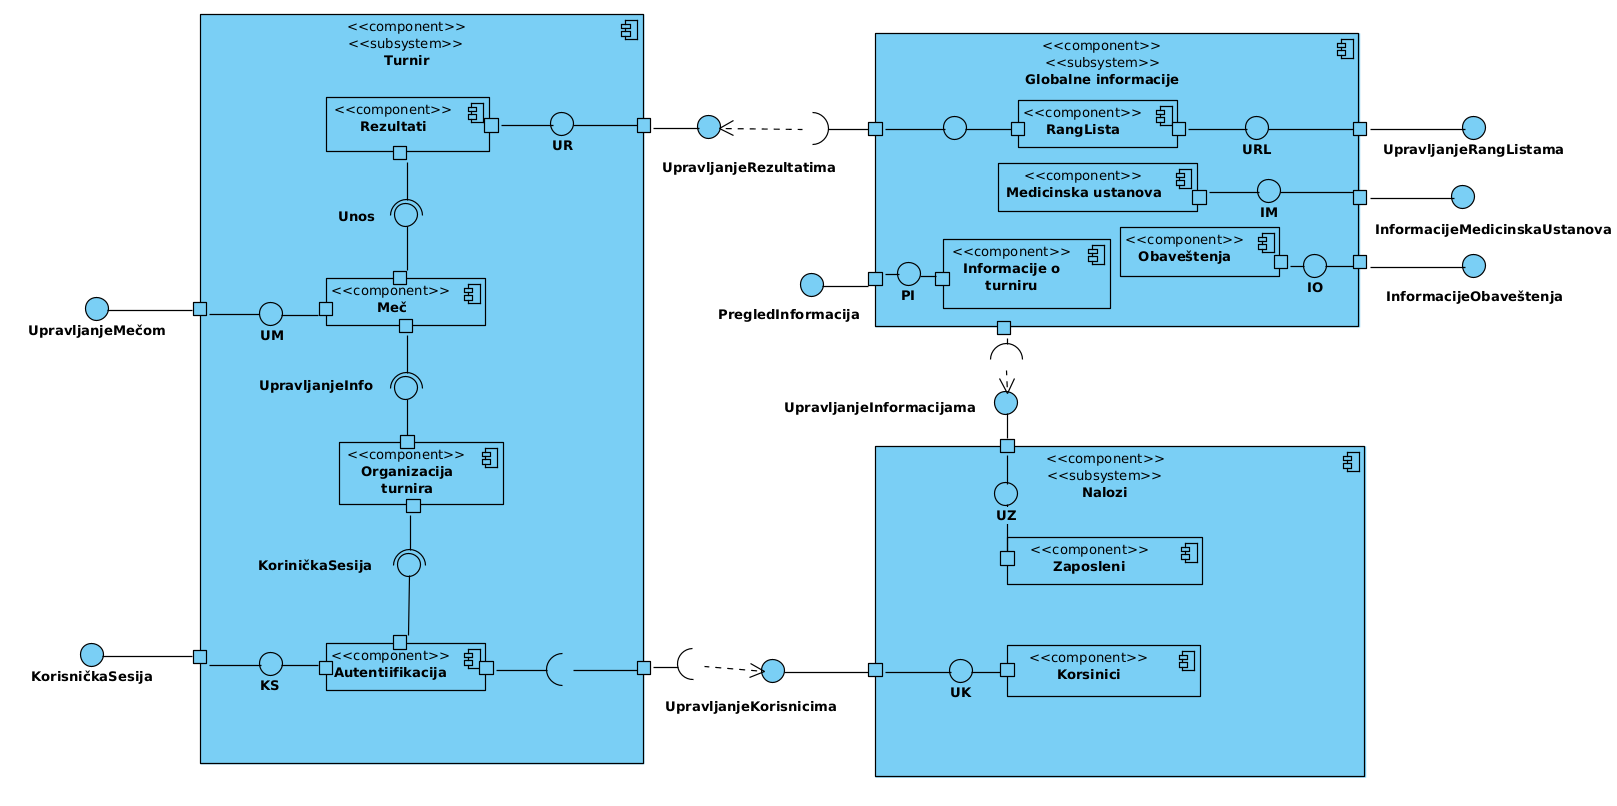
\includegraphics[scale=0.3]{Arhitektura/Dijagrami/Dijagram komponenti.png}
        \end{center}
    \caption{Dijagram komponenti}
    \end{figure}

\end{document}
